\section{The Anonymous Face and Hand Tracking Panda}

When people speak, they frequently make spontaneous hand movements that occur in synchrony with speech and naturally accompany all spoken conversation; such movements are known as gestures \cite{CLO20}. Gestures have a variety of roles in communication, learning, and comprehension for both those who observe them and those who make them. Gestures are especially effective when they resemble the thought they express, which gives them an advantage over words since it adds meaningful and distinct information while reflecting the speaker's underlying knowledge and experiences \cite{CLO20, KAN16B}. According to Feyereisen and de Lannoy \cite{FEY91}, people from all known cultures and language backgrounds gesture. Hence gestures are essential for making connections with others, although styles vary across countries.

Hand gestures, which combine with facial expressions and articulated words, play an important role in conveying our emotions. To create emotional depiction, hand movements usually combine nontrivially with facial expressions \cite{ARJ20}. It is commonly known that a person who utilizes his hands powerfully while sharing his views attracts significantly more attention than a person who only uses his voice to deliver an idea \cite{COO10, WAK18}.

As previously stated, the primary purpose of this thesis is to create a functional prototype capable of connecting people with mental health specialists anonymously, while still maintaining patient-therapist empathy. Therefore the addition of hand tracking is a critical step toward our goal in order to get deeper emotional recognition. Because, in addition to facial emotions and body posture, hands are the most significant nonverbal clues to identify specific states in others, such as anxiety states \cite{WAX97, REI22}. 

Some studies suggest that nonverbal cues may be more reliable indicators of clinical conditions than patient verbal information \cite{KNA13}. For example, research in clinical psychology has discovered that human patients' nonverbal behavior unintentionally revealed intimate information that was not given in their spoken behavior \cite{FAB06, KLE03}. Nonverbal behavior, in general, plays an important part in the establishment and maintenance of a therapeutic relationship through establishing rapport between therapists and patients in psychotherapy interactions \cite{KLE03} — in other words, therapists dedicate significant time and effort to carefully following patients' nonverbal behavior and adjusting their own nonverbal conduct in order to respond effectively and develop trust \cite{ABA21}. Furthermore, according to Abargil et al. \cite{ABA21}, through the recognition of emotions, therapists are able to adjust therapy according to the patient's nonverbal and verbal cues, and thus obtain a better outcome. Another example reveals that when describing pain, co-speech gestures convey additional information beyond that provided in speech, potentially making an essential contribution to the communication of this experience and providing hints for changing the therapy methods and results \cite{ROW16, REI22}.

\subsection{Approach}

When reviewing and testing the Anonymous Face Tracking Panda prototype, we found that the virtual avatar's ability to express themselves was limited by the lack of hand movement, which made it seem unrealistic and similar to a puppet acting. Through this finding, we questioned if the addition of hand tracking would affect or not the ability to elicit the same emotional response as human-to-human interactions (RQ1).

As previously mentioned, various researchers believe that hand gestures, in conjunction with facial expressions and articulated words, play a significant part in conveying our emotions. As a result, adding hand tracking to the current prototype is a vital step in achieving our goal of deeper emotional recognition. Because, aside from facial expressions and body posture, hands are the most important nonverbal cues for recognizing specific states in others \cite{WAX97, REI22}.

While there are a variety of ways to perform hand tracking, such as with virtual reality devices or gloves, we believe that the leap motion controller is the best option for this thesis because it is a practical and small device that does not interfere with the face recognition part.

The Leap Motion Controller (Figure 9) is a device that connects to a PC or a Mac and allows users to manipulate digital objects using hand motions. It adds a new way to interact with the digital world when combined with other hardware. Programs that interpret gesture-based computing allow users to play games, design, and learn in a hands-on manner. This device maps and tracks the human hand using an infrared scanner and sensor. This data is used to create a digital version of the hand that can manipulate digital objects in real time.

\begin{figure}[h!]
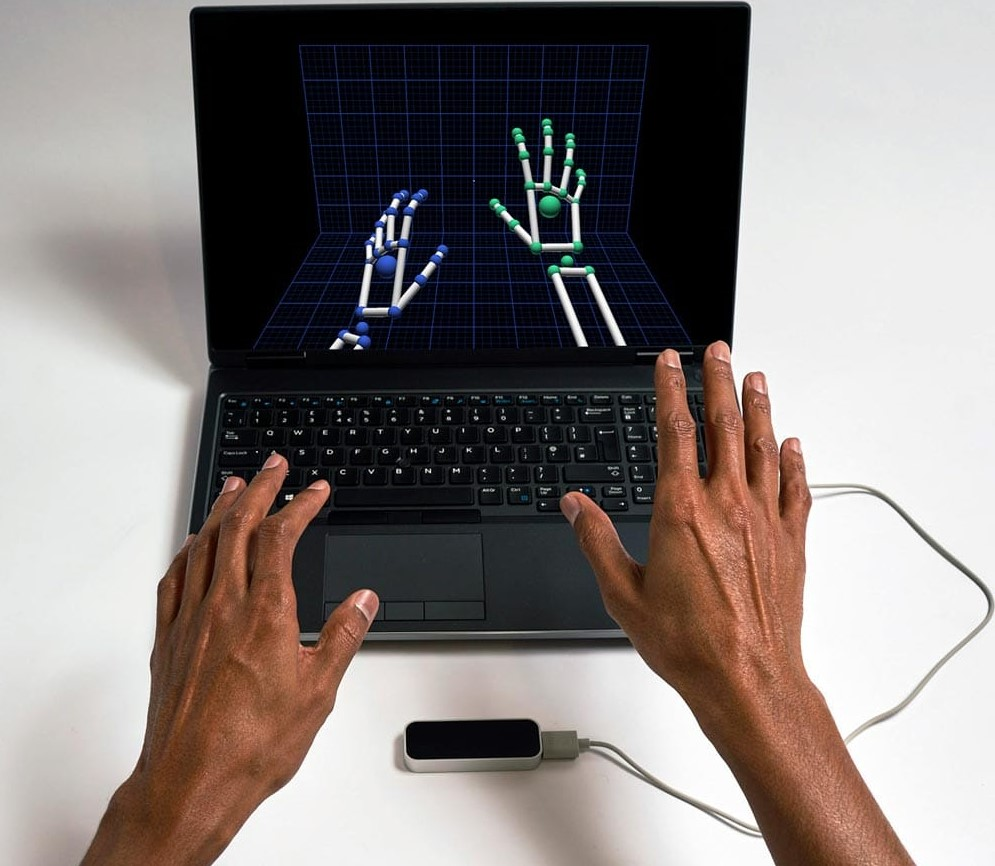
\includegraphics[width=0.6\textwidth]{figures/leapMotion.jpg}
\centering
\caption{Example of the leap motion tracking}
\end{figure}

In order to connect the existing Anonymous Panda prototype with the hand tracking part, it was necessary to use the official UE4 plugin, the Ultraleap Hand Tracking Plugin \cite{ULT}. This plugin allows Unreal developers to make use of the data obtained by incorporating Ultraleap's hand tracking data into their projects. It was designed with the intention of developing and implementing hand tracking in Extended Reality (XR) projects \cite{XR}, but with the right adjustments, it may be possible to adapt its use to other types of projects \cite{ULTG}.

\makebox[\textwidth]{\color{orange} * IN PROGRESS *}

% Meanwhile, by introducing this device, we are introducing a new limitation. The fact that, despite being more affordable than an Apple device with the TrueDepth sensor, this device is more difficult to obtain because it is sold in fewer stores.

%the sense of self-attribution of a body is called the sense of body ownership (SoBO) in the field of psychology, and the realistic the avatar, the stronger is the SoBO

\subsubsection{Challenges}

\makebox[\textwidth]{\color{red} * TO-DO *}

\subsubsection{Limitations}

\makebox[\textwidth]{\color{red} * TO-DO *}

\subsection{Methodology}

\makebox[\textwidth]{\color{red} * TO-DO *}

\subsubsection{Participants}

\makebox[\textwidth]{\color{red} * TO-DO *}

\subsubsection{Procedure}

\makebox[\textwidth]{\color{red} * TO-DO *}

\subsubsection{Hypotheses and Analyses}

\makebox[\textwidth]{\color{red} * TO-DO *}

\subsubsection{Results}

\makebox[\textwidth]{\color{red} * TO-DO *}

\subsubsection{Discussion}

\makebox[\textwidth]{\color{red} * TO-DO *}
